We use a system of differential equations to model the dynamics between the states listed in Section 2.1. The diagram of the described compartment model, with compartments and flows, is depicted on Figure \ref{fig:compartment}. \\


\begin{figure}[!h]
  \centering
  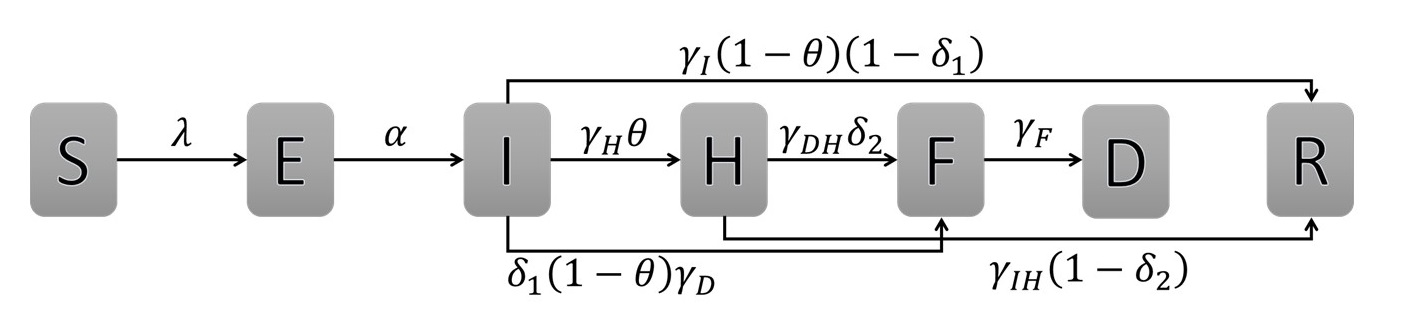
\includegraphics[width=0.7\textwidth]{compartment}
  \caption{The compartment model from Section 2.1 with flow parameters. All possible flows are specified by the arrows and parameters. We define $\lambda = \beta_{I}I+\beta_{H}H+\beta_{F}F $, a combination of the $\beta$ transmission terms shown in Table~\ref{tab:knownParameters}. } 
\label{fig:compartment} 
\end{figure}


The governing equations of the system dynamics shown above are the following:
\begin{align}
\frac{dS}{dt} &= - \frac{\beta_{I}SI+\beta_{H}SH+\beta_{F}SF}{N} \label{eqn:SD1}\\
\frac{dE}{dt} &=  \frac{\beta_{I}SI+\beta_{H}SH+\beta_{F}SF}{N}-\gamma_P E         \label{eqn:SD2}\\
\frac{dI}{dt} &=  \gamma_P E - [\gamma_{H}\theta + \gamma_{I}(1-\theta)(1-\delta_{1})+\gamma_{D}(1-\theta)\delta_{1}]I \label{eqn:SD3}\\
\frac{dH}{dt} &= \gamma_{H}\theta I - [\gamma_{HD}\delta_{2}+\gamma_{HR}(1-\delta_{2})]H \label{eqn:SD4}\\
\frac{dF}{dt} &= \gamma_{D}(1-\theta) \delta_{1} I + \gamma_{HD}\delta_{2} H-\gamma_{F} F  \label{eqn:SD5}\\
\frac{dR}{dt} &= \gamma_{I}(1-\theta)(1- \delta_{1}) I + \gamma_{HR}(1-\delta_{2}) H       \label{eqn:SD6}\\
\frac{dD}{dt} &= \gamma_{F} F  \label{eqn:SD7}
\end{align}\\
where each of the parameters are defined on Tables~\ref{tab:knownParameters} and \ref{tab:calibratedParameters}. Here $\gamma_x$ refers to $1/t_x$ for the different periods. The equations described obey total conservation, guaranteeing that the total of the compartment values remains constant. This can be seen by adding all terms on the right-hand sides, which sum to 0. 



%EQUATION DESCRIPTION


%$Accumulation = Input - Output$, in our case,
%
%\begin{equation}
%\frac{d (Accumulation)}{dt} = \frac{d (Input)}{dt} -\frac{d (Output)}{dt} \nonumber
%\end{equation}


Equation \ref{eqn:SD1} describes the change with respect to time of the susceptible population. The transition from S to E depends on $\beta_{I}SI+\beta_{H}SH+\beta_{F}SF$, which is the contact rate with the compartments I, H and F (all of which are infectious), and the respective number of value of each compartment.

Equation \ref{eqn:SD2} describes the change of the exposed compartment. This depends on the flow leaving S and the flow from E to I normalized by the incubation period $t_P$.

Equation \ref{eqn:SD3} describes the change of the infected compartment, which adds the flow from E. Flows out of compartment I include the flow from I to H, which is given by the product between the transition rate from I to H and the probability of hospitalization hospitalized; in the same way, substracting the individuals that transitions from I to R, given by  the product among the duration of infection rate, the probability a case is NOT hospitalized and the death rate of an unhospitalized case. Finally substracting the individuals that transitions from I to F , given by the product between the transition rate from Infected to Dead,  the probability a case is NOT hospitalized and the death rate of an unhospitalized case.

Equation \ref{eqn:SD4} describes the changes on the Hospitalized patients. It depends on the number of individuals that transitions from I to H, given by the  product between the transition rate from Infected to Hospitalized and the probability a case is Hospitalized;  substracting the individuals than transitions from H to D, given by the product among the transition rate from Hospitalized to Dead and the death rate of a hospitalized case, and finally, susbtracting the people that transitions from H to R, which is given by the product between the transition rate from I to R and the survival rate of an hospitalized case.

Equation \ref{eqn:SD5} describes the changes on the Funeralized compartment.  Depending on the number of individuals that transitions from I to D, which is given by the product between the transition rate from I to D, the probability a case is NOT hospitalized and the death rate of an unhospitalized case. Adding the people who transitions from H to F , which is given by the product between the transition rate from H to D and the death rate of an hospitalized case. Finally substracting the individuals who already have been buried.

Equation \ref{eqn:SD6} describes the changes on the Recovered compartment. Depending on the transition from I to R, which is given by the product between the duration of infection rate, the probability a case is NOT hospitalized and the survival rate of an Unhospitalized rate. Adding  the individuals who transitions from H to I, which is given by the product among the transition rate from I to H and the survival rate of a hospitalized case.\\

Equation \ref{eqn:SD7} describes the changes on the Funeralized compartment, which solely depends on the rate of duration of a traditional funeral.\\





%Parameter calibration
\subsection{Parameter Calibration}

The parameter values which represent biological processes ($\alpha, \gamma_{I}, \gamma_{D}, \delta_{1}, \delta_{2}$) or social customs ($\gamma_{F}$) had values listed in the previous literature \cite{Poletto2014, Webb2015}, while the parameters which represent social behavior ($\mathcal{P}=\{\beta_{I}, \beta_{H}, \beta_{F}, \gamma_{H}, \theta\}$) are site-dependent (see Tables \ref{tab:knownParameters} and \ref{tab:calibratedParameters} and Equations \ref{eqn:SD1} to \ref{eqn:SD7} for the parameter definitions). The parameters $\gamma_{DH}$ and $\gamma_{IH}$ are also unknown, but we assume the following relation with known parameters: $1/\gamma_{DH}$=$1/\gamma_{D}$-$1/\gamma_{H}$ and $1/\gamma_{IH}$=$1/\gamma_{I}$-$1/\gamma_{H}$. In this chapter, we calibrate $\mathcal{P}$ based on our systematic model (Equations 1-7) and the data of cumulative deaths in Liberia from March 2014 to July 2015 \cite{CDCData}.


\subsection{Bayesian Calibration Framework}
We use Bayesian methodology to calibrate the unknown system parameters. This method is utilized in many calibrations of complicated systems owing to its merit that little or no information of the parameter values is needed for its usage. The calibration procedure starts from choosing a distribution in the space of parameters. This distribution, the ``prior distribution" ($\mathcal{D}_0$), can be a simple distribution such as uniform or other intuitively chosen parametric distribution. Based on the available data and mathematical setup, we evaluate the likelihood weight for the samples from $\mathcal{D}_0$ with which we update the ``posterior distribution" ($\mathcal{D}_1$). Multiple updates ($\mathcal{D}_1$ to $\mathcal{D}_2$, $\mathcal{D}_2$ to $\mathcal{D}_3$, ...) facilitate a more accurate distribution.

To calibrate the unknown parameters ($\mathcal{P}$), we started from an uniform prior distribution in the range determined based on numerical exploration and previous literature (see Table \ref{tab:PriorRanges}) \cite{Rivers2014}. \\

\begin{table}[ht]
\centering % used for centering table
\begin{tabular}{c c c c c}
\hline\hline %inserts double horizontal lines
$\beta_{I}$ & $\beta_{H}$ & $\beta_{F}$ & $\gamma_{H}$ & $\theta$ \\ [0.5ex]
\hline % inserts single horizontal line
$(0,0.5)$ & $(0,0.5)$ & $(0,1)$ & $(2,7)$ & $(0,0.5)$ \\ [0.5ex]
\hline
\end{tabular}
\caption{Range of the prior parameter space} % title of Table
\label{tab:PriorRanges}
\end{table}


To each random choice ($\mathcal{P}_0$) from the prior distribution, we assigned likelihood weight by comparing the World Health Organization (WHO) data reports ($\mathcal{D}_R$) to the data simulated with $\mathcal{P}_0$ ($\mathcal{D}_S$) from the systems-based model. Repeating this method, we build the posterior distribution for $\mathcal{P}$. In this methodology, we provide multiple likely parameter sets, rather than a single best fit, by listing the mean as well as the standard deviation of suggested parameter values. The algorithm for the parameter calibration is:

Step 1) Choose a random $\mathcal{P}_0$ from the prior distribution.

Step 2) Solve the deterministic system (Equations 1-7) with $\mathcal{P}_0$ and given initial value $\{S_0,E_0,I_0,F_0,D_0,R_0\}$, then evaluate $\mathcal{D}_S=\{D(t_i)\}$ for all dates $\{t_i\}$ corresponding to the cumulative death data ($\mathcal{D}_R$).

Step 3) Evaluate likelihood of $\mathcal{P}_0$: $\exp\left(-\lVert\mathcal{D}_R-\mathcal{D}_S\rVert_2/\lVert\mathcal{D}_R\rVert_2\right)$.

\emph{Repeat Steps 1-3 many times to generate {parameter and likelihood} estimates. Generate the posterior distribution using these weights.}

\subsubsection{Results and validation}
We applied our systematic model and calibration method to the Ebola spread in Liberia during 2014-2015. Two sets of cumulative mortality data (pre-intervention and post-intervention) are used to calibrate pre- and post-intervention parameters, respectively. We assume that about a forth (1 million) of Liberia's total population (4.3 million \cite{LiberiaPop}) are involved in the model, and that the rest of the population are not at risk due to geographical location or behavioral reasons. For the calibration of pre-intervention parameters, we used the data from 176 days (March 2014 to September 2014) and initial values $\{S_0,E_0,I_0,F_0,D_0,R_0\}$=$\{10^6-1,0,1,0,0,0\}$ assuming that the initial outbreak started from a single infected person. The calibration of post-intervention parameters is based on the data from 306 days (September 14 to July 15) and initial values $\{S[176],E[176],I[176],F[176],D[176],R[176]\}$ which are evaluated from the calibrated parameter means $\mathcal{P}$ for pre-intervention. Each calibration used 10,000 random samples.

\begin{table}[ht]
\centering % used for centering table
\begin{tabular}{c  c c}
\hline\hline %inserts double horizontal lines
Parameter &  Pre-Intervention  & Post-Intervention \\ [0.5ex]
 & (Mar 2014 to Sept 2014) &  (Sept 2014 to July 2015)\\ [0.5ex] % inserts table
% inserts table
%heading
\hline % inserts single horizontal line
{Contact Rate, Community  (${\beta_{I}}$) }& {0.148 (0.0953)} & {0.0446 (0.0338)}  \\
Contact Rate, Hospital  ($\beta_{H}$) & 0.235 (0.143) & 0.0877 (0.0563) \\
Contact Rate, Funeral  ($\beta_{F}$) & 0.465 (0.287)& 0.283 (0.208) \\
Time until Hospitalization (${t_{H}}$) & 4.49 (1.44) days & 4.63 (1.43) days  \\
Time from Hospitalization to Death (${t_{HD}}$) & 3.51 (1.44) days & 3.51 (1.43) days  \\
Time from Hospitalization to Recovery (${t_{HR}}$) & 5.51 (1.44) days & 5.51 (1.43) days \\
Probability a Case is Hospitalized ($\theta$) & 0.248 (0.142) & 0.233 (0.145) \\
[1ex]
\hline
\end{tabular}
\caption{Calibrated parameters for Ebola epidemic in Liberia. Posterior mean and standard deviation (in parentheses) are listed for pre-intervention and post-intervention calibrations.}%For comparison, the evaluated values through least-square optimization \cite{Rivers2014} are in 4th column.} % title of Table
\label{tab:calibratedParameters}
\end{table}

Calibration results are shown in Table \ref{tab:calibratedParameters}. By observing the posterior mean of the two calibrations, we conclude that our calibration reasonably predicts decreased transmission rates ($\beta_I$, $\beta_H$, $\beta_F$) post-intervention. See Figure \ref{fig:BetaStepFunction} for the differences of these parameters; the step function pictured is used when running the systems model. The parameters for time until hospitalization ($\gamma_H$) and the probability a case hospitalized ($\theta$) were calibrated to have the same approximate value pre- and post-intervention. This may be reasonable if, for example, the hospital capacity  insufficient to handle the increasing number of cases. It also tells shows that the system dynamics are more sensitive to the changes in {$\beta_I$, $\beta_H$, $\beta_F$} compared to the changes in {$\gamma_H$, $\theta$}.


We validated our calibration in Figure \ref{fig:Cumulative _Death}, which shows a good fit between the used cumulative death data and the systems model using the calculated parameter means.


\begin{figure}[!h]
  \centering
  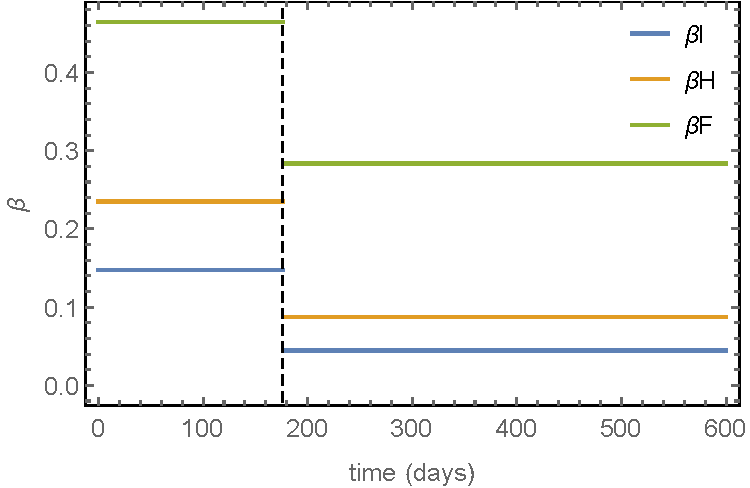
\includegraphics[width=0.7\textwidth]{BetaStepFunction.pdf}
  \caption{$\beta$ step function} 
\label{fig:BetaStepFunction} 
\end{figure}


\begin{figure}[h]
  \centering
  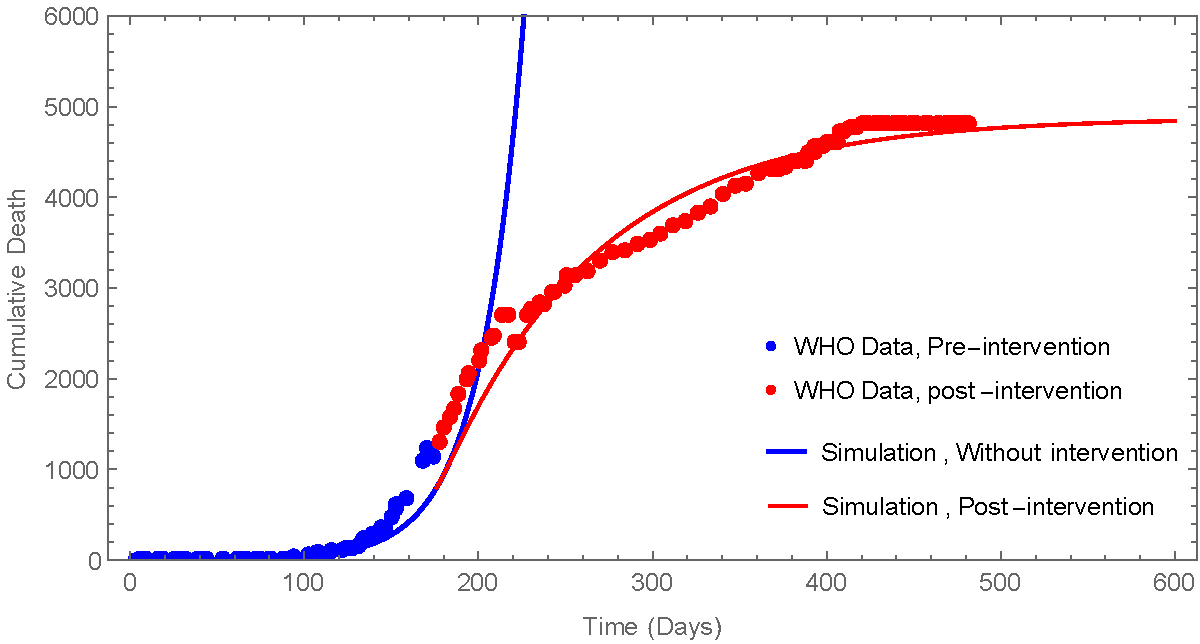
\includegraphics[width=1\textwidth]{ValidationPlot.pdf}
  \caption{Validation of calibration. Dots represent cumulative death data and the lines represent simulation based on mean posterior parameters. (Blue) - pre intervention and (red) - post treatment.}
\label{fig:Cumulative _Death}
\end{figure}




\subsection{Simulation}
 Insight Maker is a powerful online tool used to model and simulate complex systems. It utilizes different approaches, such as System Dynamics, Agent-Based Modeling and imperative programming. Insight Maker permits  construction of a graphical model to forecast the system response \cite{FortmannRoe}. We used the InsightMaker platform to prototype our model and simulate stepping forward through time. More details about the platform and its functionality can be found in Fortmann-Roe's review \cite{FortmannRoe}. The platform uses a fourth-order Runge-Kutta differential equation solver for the system dynamics model and  first order Euler approximation for the Agent-Based model.\\

\noindent The compartment S was initialized with a value of 999999, and the compartment I with 1, meaning that there is an infected individual per every million of individuals, the rest of the compartments were set to zero as an initial condition. The flow between the compartments is given in the equations and all the other parameters were initialized as shown in Tables   \ref{tab:knownParameters} and \ref{tab:calibratedParameters}.  As mention at the beggining of the section, the parameters were calibrated in two stages, before and after the international intervention. According with the time frame proposed, the change in the parameters was also implemented on Insight Maker. The links to the online models can be found on \cite{IM_AI} and  \cite{IM_BI}.\\ 


% RESULTS AND DISCUSSION
%
%No intervention
\noindent After modeling the system with the parameters before the intervention, it can be observed in Figure \ref{fig:LB_IM_NoIn} how the total population decreases to 46.46\%  if there is no intervention and the each of the parameters continue to be the same. The number of susceptible individuals exponentially decays, converging to 7\% of the population, while exposed, infected, hospitalized and funeral comparments converges to zero; finally, after the system stabilizes, the final proportion of deaths would be 53.53\% \\

\begin{figure}[!h]
  \centering
  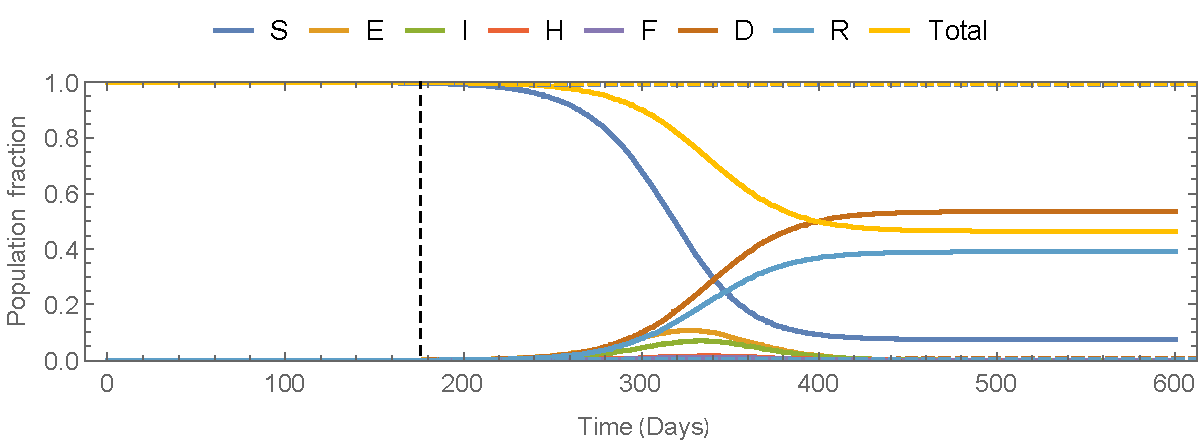
\includegraphics[width=1\textwidth]{SEIPlot.pdf}
  \caption{Simulation results using the parameters of the first stage (Mar 2014  to Sept 2014) and assuming no intervention}
\label{fig:LB_IM_NoIn} 
\end{figure}

%Intervention 
\noindent As mentioned before, five parameters were calibrated for the second stage of the Ebola Outbreak, namely, community contact rate ($\beta_I$), hospital contact rate ($\beta_H$), funeral contact rate ($\beta_F$), time until hospitalization ($\gamma_H$) and probability a case is hospitalized ($\theta$). Figure \ref{fig:LB_IM_In} A. shows that there is not much change in the Total population and susceptible compartment, meaning that the virus was controlled;  Figure \ref{fig:LB_IM_In} B focuses on E, I, R, H , F and D compartments, showing that the international intervention causes a dramatic change in the behavior of such compartments.


\begin{figure}[h!]
  \centering
  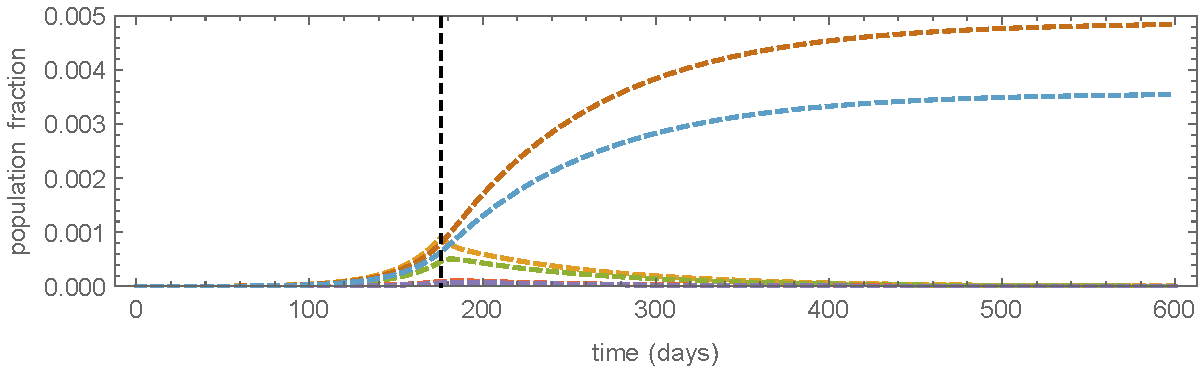
\includegraphics[width=1\textwidth]{SEIPlotIntRescale.pdf} 
\caption{ Parameters of the second stage ( Sept 2014 to July 2015).} 
\label{fig:LB_IM_In} 
\end{figure}





%Comparing with WHO data

\noindent Finally, a comparison between the proposed model and World Health Organization data is shown in Figures \ref{fig:LB_IM_WHO} and \ref{fig:LB_IM_WHO2}. As depicted in Figure \ref{fig:LB_IM_WHO}, there is a good fitting of our model with the data reported by WHO. Figure \ref{fig:LB_IM_WHO2} shows  the reported WHO data before and after intervention, the results of our model before and after intervention and the forecast for the coming months, predicting that after the system reaches an equilibrium, the proportion of deaths in Liberia product of the EVD would be 5.07\% approximately.



\begin{figure}[h!]
 \centering 
 \begin{subfigure}[b]{0.38\textwidth}
  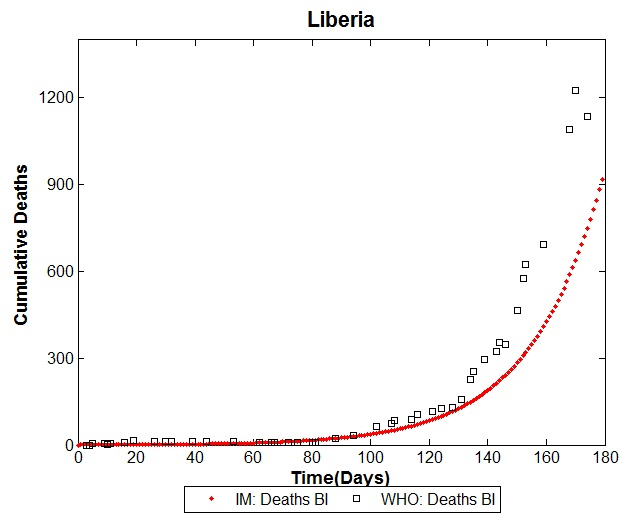
\includegraphics[width=\textwidth]{LB_BI_SD_WHO_IM} \caption{BI: Before Intervention Parameters (March 2014  to Sept 2014)} \label{fig:LB_BI_SD_WHO_IM} \end{subfigure}
 %
 \hspace{.1cm}
\begin{subfigure}[b]{0.38\textwidth}
 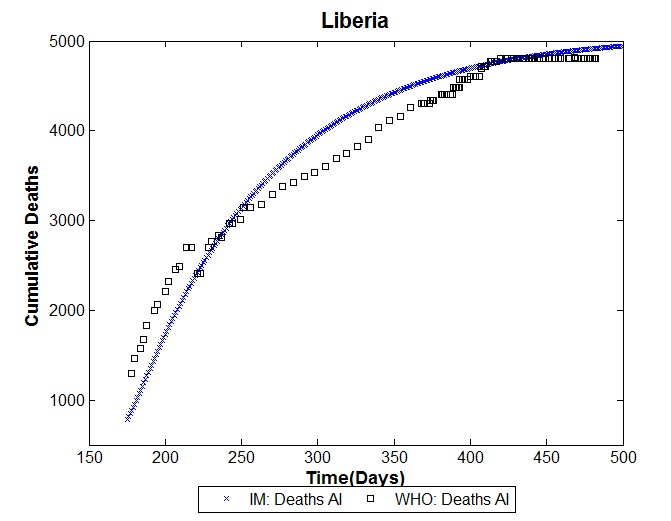
\includegraphics[width=\textwidth]{LB_AI_SD_WHO_IM} \caption{AI: After Intervention Parameters  ( Sept 2014 to July 2015).} \label{fig:LB_AI_SD_WHO_IM} \end{subfigure} 
\caption{Comparison between World Health Organization (WHO) data and Insight Maker (IM) results for cumulative deaths (D)}
\label{fig:LB_IM_WHO} 
\end{figure}



\begin{figure}[!h]
  \centering
  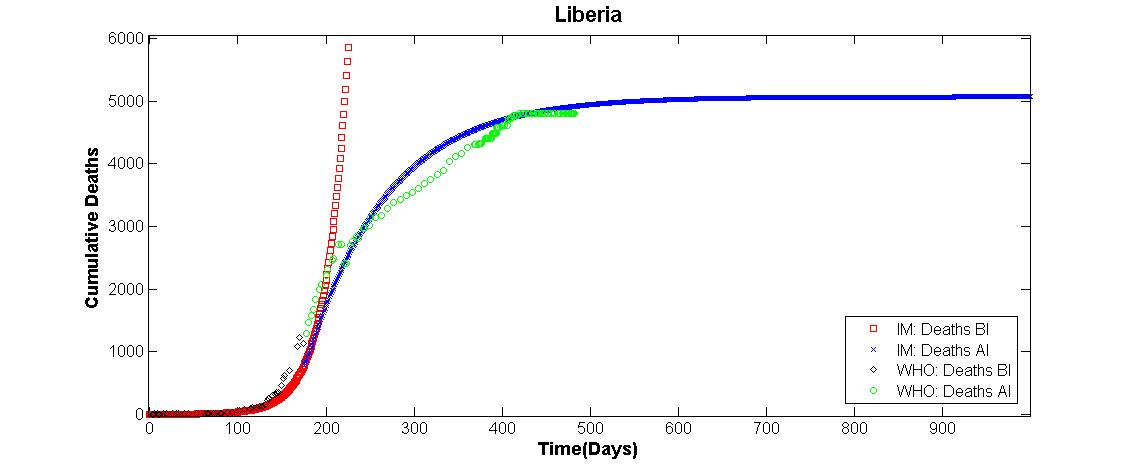
\includegraphics[width=1\textwidth]{LB_Int2_SD_WHO_IM}
  \caption{ Comparison between World Health Organization (WHO) data and Insight Maker (IM) results using the parameters before intervention (BI) and after intervention (AI), for the cumulative deaths (D).}
\label{fig:LB_IM_WHO2} 
\end{figure}


Figure \ref{fig:PhasePortrait} shows another visualization of our simulation on 2 dimensional space of $S+R$ vs. $D$. By watching the phase portrait in the figure, we can see that the fraction of survived population after outbreak $S+R$ converges to $46\%$ and dead people $D$ converges to $54\%$ without intervention. However, with intervention on 176th day, the $S+R$ and $D$ converge to $99.5\%$ and $0.487 \times10^{-3}\%$, respectively. The significant effect of intervention observed here can be analyzed by the basic reproduction number ($R_0$). $R_0$ is a indicator to tell if the infection will spread (if $R_0>1$) or die out (if $R_0<1$) eventually in the population. Evaluated Based on (reference), $R_0$ is $1.99 (>1)$ before intervention. However, it has been changed with after intervention to $0.786(<1)$.


\begin{figure}[h!]
 \centering 
 \begin{subfigure}[b]{0.38\textwidth}
  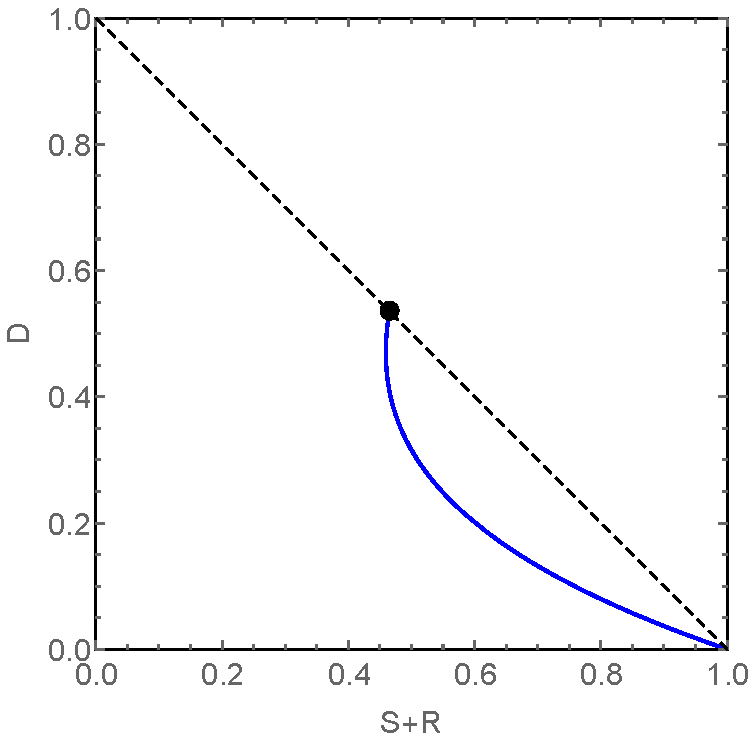
\includegraphics[width=\textwidth]{PhasePortraitSRnD1.pdf} \caption{Full scale} \label{fig:PhasePortraitA} \end{subfigure}
 %
 \hspace{.1cm}
\begin{subfigure}[b]{0.38\textwidth}
 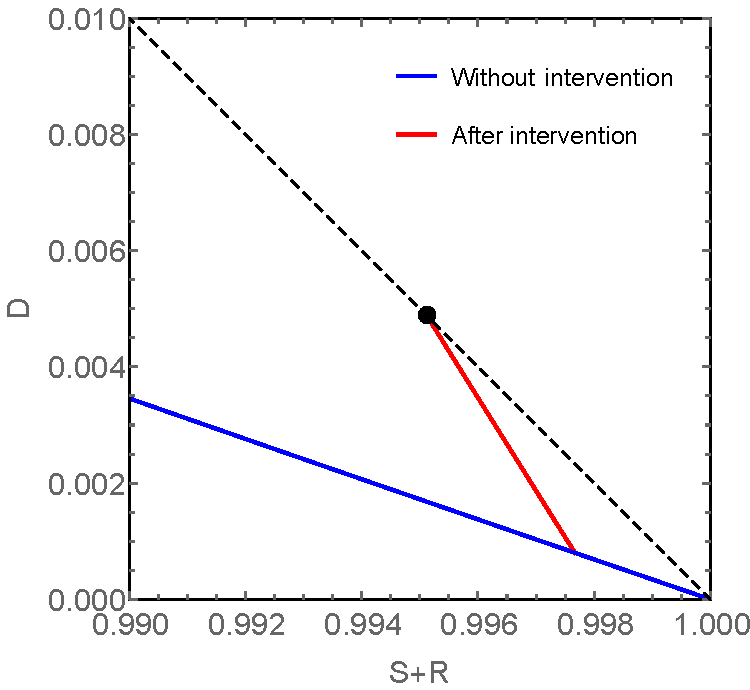
\includegraphics[width=\textwidth]{PhasePortraitSRnD2.pdf} \caption{Rescaled plot of (a) to enlarge right bottom corner} \label{fiig:PhasePortraitB} \end{subfigure} 
\caption{Projection of phase portrait to (Susceptible + Recovered, Dead) space. (Blue) - without intervention, (Red) - with intervention, (Dots) - where the phase converges (equilibrium)}
\label{fig:PhasePortrait} 
\end{figure}





